% Reviewer (1)% Reviewer (2)% Reviewer (3)
\documentclass[10pt]{article}
\usepackage{a4wide}
\usepackage{xcolor}
\usepackage{color,soul}
\usepackage{mdframed}
\usepackage{caption}
\captionsetup[table]{skip=10pt}
\usepackage{enumerate}
\usepackage{url}
\usepackage{textcomp}
\usepackage{amsmath}
\usepackage{bbm}


\newcommand{\rev}[1]{{\bf Rev.\,\##1}}
\newcommand{\latexdiff}{\texttt{latexdiff}}
\newcommand{\chk}[1]{\textcolor{red}{#1}}
\newcommand{\reviewer}[1]{\textbf{#1}}
\newcommand{\answer}[1]{#1}
\newcommand{\us}{\char`_}

\newcommand{\MT}[1]{\textcolor{blue}{MT: #1}}

\newcommand{\ccnsim}{ccn\ensuremath{\mathcal{S}}im} % \'a la rossini ;)
\newcommand{\akaroa}{Akaroa2\textcopyright\ }
\usepackage{textcomp}
\newcommand{\textapprox}{\raisebox{0.5ex}{\texttildelow}}

\newcommand{\firstfakeieeepar}[1]{\noindent{\textit{#1.}}}
\newcommand{\firstfakeacmpar}[1]{\noindent{\textbf{#1.}}}
\newcommand{\fakeieeepar}[1]{~\\\noindent{\textit{#1.}}}
\newcommand{\fakeacmpar}[1]{\vspace{2 mm}\noindent{\textbf{#1.}}}
\newcommand{\fakeacmparnobold}[1]{\noindent{\textit{#1.}}}
\newcommand{\fakesubsection}[1]{\fakeieeepar{#1}}
\newcommand{\firstfakesubsection}[1]{\firstfakeieeepar{#1}}

\usepackage{tikz}

\newcommand\encircle[1]{%
  \tikz[baseline=(X.base)] 
    \node (X) [draw, shape=circle, inner sep=0] {\strut #1};}


%\renewcommand{\ccnsim}{ccnSim}

%\DeclareRobustCommand{\hlg}[1]{{\sethlcolor{cyan!10}\hl{#1}}}
\newcommand{\colorboxg}[1]{{\colorbox{gray!20}{#1}}}

%========================================================================
%  to make missing refs really standout
%------------------------------------------------------------------------
% http://www.latex-community.org/forum/viewtopic.php?f=5&t=13654
 \newcommand*{\missingreference}{\colorbox{red}{?reference?}}
 \newcommand*{\missingcitation}{\colorbox{red}{?citation?}}
 \makeatletter
 \def\@setref#1#2#3{%
   \ifx#1\relax
    \protect\G@refundefinedtrue
    \nfss@text{\reset@font\missingreference}%
    \@latex@warning{Reference `#3' on page \thepage \space
              undefined}%
   \else
    \expandafter#2#1\null
   \fi}
 \def\@citex[#1]#2{\leavevmode
   \let\@citea\@empty
   \@cite{\@for\@citeb:=#2\do
    {\@citea\def\@citea{,\penalty\@m\ }%
     \edef\@citeb{\expandafter\@firstofone\@citeb\@empty}%
      \if@filesw\immediate\write\@auxout{\string\citation{\@citeb}}\fi
      \@ifundefined{b@\@citeb}{\hbox{\reset@font\missingcitation}%
       \G@refundefinedtrue
        \@latex@warning
          {Citation `\@citeb' on page \thepage \space undefined}}%
        {\@cite@ofmt{\csname b@\@citeb\endcsname}}}}{#1}}
 \makeatother 
%========================================================================
%  to make missing refs really standout
%------------------------------------------------------------------------



\begin{document}

{\centering 
	{\Large {\bf Caching}}\\
	{\large TBD}\\[10pt]
}

\MT{Write a small introduction that explains the content of the TP.}

\section*{PART 1 - Caching: What, Why, and How}

\MT{Explain: (i) what does it mean to ``cache a content''; (ii) why (how the hit ratio influences the user experience) and where it is used; (iii) which factors contribute to caching performance (i.e., replacement and admission policies, catalog properties like content popularity, request model, and so on.)}

...

The \emph{hit ratio} $h$, and so the resulting user experience connected to the performance of a caching system, is the result of multiple factors interplaying with each other, as shown in Fig. \MT{Add a figure with a sum of all factors giving the final hit ratio}. Well known classes of each factor are listed in the following.

\fakeacmpar{Content Popularity}
The context a caching system is used in, and especially \emph{how} requests are issued for contents identified by a particular  \emph{popularity distribution}, represents one of the influencing factors for the final hit ratio $h$.
\begin{itemize}
\item \textbf{Zipf's law} 

It is considered as the de facto popularity distribution (along with Weibull and Mandelbrot-Zipf ones) that best approximates the dynamics of common Internet services, from popularity of requested contents in a P2P network or in a CDN, to distribution of requests for websites, or popularity of videos in a streaming platform. 

In particular, denoting with $M$ the \emph{catalog cardinality}, and with $1 \le i \le M$ the rank of the $i$-th most popular content, the probability of requesting the content with rank $i$ is expressed as:
\begin{equation}\label{zipf}
P(X=i)=\frac{i^{-\alpha}}{B}.
\end{equation}
where $B=1/\sum_{j=1}^M{j^{-\alpha}}$, and $\alpha > 0$. 

Clearly, the value of the Zipf exponent $\alpha$ plays a paramount role in determining the caching performance; indeed, the percentage of requests directed to the $C$ most popular contents, i.e., $P(C)=\sum_{i=1}^C{P(X=i)}$, heavily varies with $\alpha$. 
For large values of $\alpha$, e.g., $\alpha=2$, and supposing a catalog with a cardinality of $M=10^8$ contents, $C=12$ represents the content correspondent to the 95-th percentile of requests, meaning that 95\% of requests are directed towards only the $C=12$ most popular contents (as $\sum_{i=1}^{12}{P(X=i)} > 0.95 \ \ for \ \ \alpha=2$). At the same time, with $\alpha=0.8$, for example, the head of the catalog for which the 95\% of requests is directed becomes much wider, being $C=$ \MT{complete}.
It can be concluded that the higher $\alpha$, the smaller the size of the cache needed to guarantee a certain hit ratio $h$.   

It is worth noticing, also, that the whole Internet traffic is made of a mixture of different ``types'' of traffic (Web, P2P, Video, etc.), each one with a specific set of parameters, content popularity (expressed in terms of request frequency) being one of them. This is the reason why there is neither a single $\alpha$ value that characterizes all the scenarios above, nor a broad consensus on the particular $\alpha$ that needs to be use to model each type of traffic. Empirical studies have tried to provide intervals for each application: for example, for Web and File Sharing traffic $\alpha \in [0.6,0.85]$, for VoD $\alpha \in [0.65,1]$, and for UGC $\alpha \ge 2$ \cite{DraftPentikousis:16}.       
\end{itemize}

\fakeacmpar{Temporal Locality}
The temporal dynamics of popularity, i.e., how requests are distributed in time, complement the information provided by popularity distribution, which expresses only the number of requests submitted for each content, without describing how these requests are distributed in time. This aspect is of primary importance when considering the performance of caching schemes since the ordering of the requests obviously affects the contents that will be stored inside the cache. 
There exists several models used to characterize the pattern of requests arriving at a cache:
\begin{itemize}
\item \textbf{Independent Reference Model (IRM)}

This model, widely adopted in the literature due to its simplicity, is based on the following fundamental assumptions: i) users request items from a fixed catalog of $M$ objects; ii) the probability $P(X=m)$ that a request is for object $m$, $1 \le m \le M$, is constant (i.e., the object popularity does not vary over time) and independent of all past requests, generating an i.i.d. sequence of requests.
It results that the IRM completely ignores all temporal correlations in the sequence of requests (aka temporal locality), i.e., the fact that, if an object is requested at a given point in time, then it is more likely that the same object will be requested again in the near future (a characteristic that increase the hit ratio $h$ of a cache).

\item \textbf{Shot Noise Model (SNM) \cite{garetto15infocom}}

The basic idea is to represent the overall request process as the superposition of many independent processes (shots), each referring to an individual content. Specifically, the arrival process of requests for a given content $m$ at a cache is described by an inhomogeneous Poisson process of intensity $V_m h(t - t_m)$, where $V_m$ denotes the average number of requests attracted by the content, $t_m$ is the time instant at which the content enters the system (i.e., it becomes available to the users), and $h()$ is the (normalized) ``popularity profile'' of content $m$. The SNM models, in this way, the evolution of content popularity over time.
\end{itemize}

\fakeacmpar{Spatial Locality}
It refers to the way requests are geographically distributed throughout the network. 
Being able to characterize request patterns in different areas of the network might help avoiding redundant traffic in the network itself; indeed, if requests are highly localized in some areas of the entire network, then similar requests can be more efficiently served with mechanisms such as caching.

\fakeacmpar{Replacement Policy}
Since caches have a limited amount of space to store contents (which we suppose being equal to $C$ contents), we need a \emph{replacement policy} to decide which content needs to be evicted when the cache is full and a new content needs to be stored. 
Among several techniques, the most adopted and studied ones are:
\begin{itemize}
\item \textbf{LFU}: in its classic implementation, a \emph{Least Frequently Used} cache keeps track of the access frequency by assigning a counter to each stored content, and evicting the one with the lowest counter when the cache is full. Furthermore, if the content popularity is known a priori, a LFU cache can be implemented by statically storing the $C$ most popular contents, thus providing optimal performance under IRM. However, a pure LFU system is discouraged in real contexts with evolving popularity (e.g., newly cached items with low counters might be soon evicted even though they might be required frequently thereafter). 
\item \textbf{LRU}: a \emph{Least Recently Used} cache will evict the content that has not been requested for the longest time, in case a new content needs to be inserted in the cache, and there are already $C$ contents stored in it. This means that each time a cached content is requested, its timer is updated. A LRU cache provides the best compromise between performance and easy implementation.   
\item \textbf{FIFO}: in this case, the timer of cached contents is not updated in case of a cache hit; as a consequence, the content that has been inserted since the longest time is evicted if the cache is full.
\item \textbf{RANDOM}: the content to be evicted in case of a full cache is selected randomly.
\end{itemize}

\fakeacmpar{Admission Policy}
The effective storage of a newly arrived content inside the cache can be regulated by an \emph{admission policy}, which might be related or not to the ``position'' of the cache itself inside the whole network topology.  
The most diffused techniques are:
\begin{itemize}
  \item \textbf{LCE}: with \emph{Leave Copy Everywhere}, a newly arrived content is aways cached, if not already stored inside the cache.
  \item \textbf{LCP}: \emph{Leave Copy Probabilistically} adds a filter to LCE, in the sense that a newly arrived content will be cached only with probability $p$, a parameter that can be set in order to change the caching behavior and reduce the so called \emph{cache pollution} (i.e., the worthless caching of unpopular contents). 
  \item \textbf{2-LRU}: a more affective way than LCP to reduce cache pollution is provided by this strategy \cite{martina14infocom}; before the physical cache, where actual objects are stored, there is a second cache where only content IDs of incoming requests are stored following a LRU policy. Therefore, only contents whose ID is found in the first cache are then cached in the physical one when fetched from upstream nodes. This provides a self-tuning filter that reduces cache pollution and which can cope with the temporal evolution of content popularity.     
  \item \textbf{LCD}: in a hierarchical network of caches, the \emph{Leave Copy Down} strategy leaves a copy of the requested content only inside the cache which is one hop below the cache the content has been found in. 
\end{itemize}

\section*{PART 2 - Cost and errors of computing Cache Hit Ratio $h$}
With notions of PART 1, we are now ready to go one step further and have a quick overview of the available analytical tools used to compute the \emph{cache hit ratio} $h$. 
In particular, we are interested in their computational complexity and in assessing potential errors that can be introduced when relying on simplifications. 
Due to the numerous and diverse scenarios that might result from the combination of the different factors seen above, in this TP we will make the following assumptions: \\ (i) we consider a system composed by a \emph{single cache} under \\ (ii) an IRM request model, and \\ (iii) we focus on the specific aspect of \emph{replacement policies}, considering LFU and LRU as case studies.  

\fakeacmpar{LFU}
As seen in PART 1, the quantile of the Zipf distribution for an object of rank $C$ of a catalog with cardinality $M$ can be written as:
\begin{equation}\label{quantile}
P(C)=\frac{\sum_{k=1}^C{1/k^\alpha}}{\sum_{k=1}^M{1/k^\alpha}},  
\end{equation}

which also represents the aggregate rate for the $C$ most popular contents.
Considering that a single LFU cache with size $C$ statically stores the $C$ most popular contents, it results that (\ref{quantile}) also corresponds to the \emph{cache hit ratio} $h$ of that cache:

\begin{equation}\label{hit_lfu}
h_{LFU} = P(C)
\end{equation}

For big values of $M$, (\ref{hit_lfu}) becomes computationally complex. However, except for $\alpha > 1$, it is possible to find a closed form expression for $h_{LFU}$ by using some simplification. 

\begin{itemize}
  \item $\alpha = 1$
  
  In this case, numerator and denominator of \ref{quantile} correspond to the Harmonic numbers $H_C = \sum_{k=1}^C  1/k$ (and $H_M$), which are known to be well approximated asymptotically by a logarithmic function, since
  \begin{align}
  \lim_{X\rightarrow \infty} H_X  - ln(X) = \gamma ,
  \end{align}
  \noindent where $\gamma\approx 0.57$ is the Euler-Mascheroni constant. Hence, in the large $C$ and $M$ regime, we have:
  \begin{align}\label{eq:lfu_approx}
  h^{app}_{LFU}\approx ln(C)/ln(M). 
  \end{align}

  Fig. \ref{fig:lfu_approx_a1} compares the true hit ratio $h$ (\ref{hit_lfu}) for a fixed size cache $C$ and varying $M$ against its approximation (\ref{eq:lfu_approx}). It can be noticed that despite (i) this approximation works as better as $C$ and $M$ increase, (ii) a non-negligible error persists in every case. There is, indeed, a compromise to accept between computational ease and prediction error.  

  \item $\alpha < 1$

  In this particular case, the harmonic number can be approximated as:
  \begin{equation}
  H_C \approx \int_{1}^{C} 1/x^{\alpha} dx = \frac{x^{(1-\alpha)}}{1-\alpha} = \frac{C^{(1-\alpha)}}{1-\alpha}
  \end{equation}
  It follows that:
  \begin{equation}\label{eq:lfu_approx_ah1}
  h^{app}_{LFU} \approx \frac{C^{(1-\alpha)}}{M^{1-\alpha}} = \left(\frac{C}{M}\right)^{1-\alpha}
  \end{equation}

  It is worth noticing that the approximation (\ref{eq:lfu_approx_ah1}) comes with a higher absolute error (i.e., $|h_{LFU}-h^{app}_{LFU}|$) with respect to the approximation (\ref{eq:lfu_approx}) \MT{Insert an explicative plot}.
  

 \begin{figure}[t] 
   \centering
     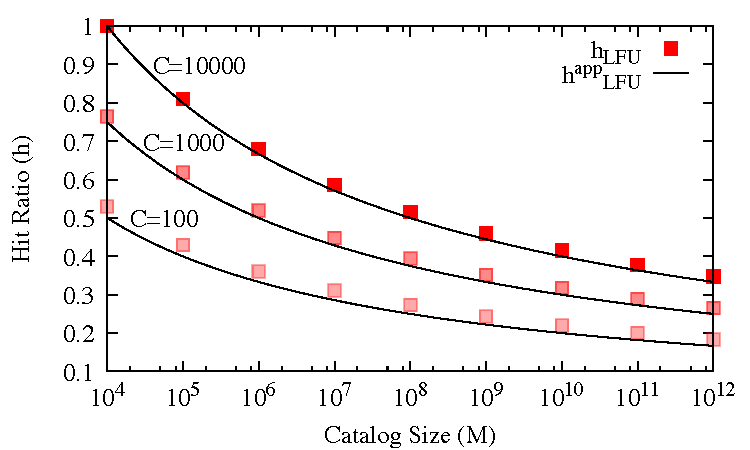
\includegraphics[width=0.7\textwidth]{QuellaSporcaDozzina.pdf}
   \caption{Single LFU cache with fixed size $C$ and varying cardinality $M$. True hit ratio $h_{LFU}$ vs its approximation $h^{app}_{LFU}$ for $\alpha=1$.}
   \label{fig:lfu_approx_a1}
\end{figure} 

\end{itemize}

\fakeacmpar{LRU}
The computational complexity of exactly predicting the cache hit ratio $h$ for a single cache with LRU replacement policy lies in the exponential growth with cache size $C$ or with catalog cardinality $M$ \cite{King:71}, which makes impossible to obtain the final results in a reasonable amount of time for real scenarios (i.e., with $M \ge 10^8$).
Therefore, the only feasible way to obtain a reference point is by simulation. 
However, plenty of models and approximations have been proposed so far, among which Che's approximation \cite{wang02jsac_hierarchical} represents the most adopted and effective one. It was initially conceived for a single cache with LRU replacement policy and IRM traffic, and then successively extended for other traffic types, replacement and admission policies \cite{martina14infocom}.

\begin{itemize}
  \item \textbf{Che's Approximation \cite{wang02jsac_hierarchical}}

  The core intuition is that of considering the eviction time $T_C(m)$ for content $m$, with $1 \le m \le M$, as if it was a constant value $T_C$, known as ``characteristic time'', independent of the content $m$. In particular, $T_C(m)$ can be considered for a cache of size $C$ as the time needed before $C$ distinct contents (excluding $m$) are requested, i.e., the time since the last request (for $m$) after which content $m$ will be evicted (provided that it has not been requested in the meanwhile).  

  Che's assumption greatly simplifies the analysis of caching systems because it allows to decouple the dynamics of different contents: the interaction among contents is summarized by $T_C$, which acts as a single primitive quantity representing the response of the whole cache to an object request.

  Formally speaking, Che's approximation states that an object $m$ is in the cache at time $t$, if and only if a time smaller than $T_C$ has elapsed since the last request for object $m$, i.e., if at least a request for $m$ has arrived in the interval $(t - T_C, t]$. Under the assumption that requests for object $m$ arrive according to a Poisson process of rate $\lambda_m$, the time-average probability $p_{in}(m)$ that object $m$ is in the cache is given by:
  \begin{equation}\label{pin}
  p_{in}(m) = 1 - e^{-\lambda_m T_C}
  \end{equation}

  It is worth noticing that $p_{in}(m)$ represents also the hit probability $p_{hit}(m)$ (thanks to PASTA's property), i.e., the probability that a request for content $m$ finds content $m$ inside the cache. 
  Denoting  with $\mathbbm{1}_{\text{\{A\}}}$ the indicator function for event $A$, we have that by construction, cache size $C$ must satisfy:%
  \begin{equation}\label{TC}
  C=\mathbbm{E}\left[ \sum_m \mathbbm{1}_{\{\text{$m$ in cache at t}\}}\right]= \sum\limits_{m} p_{in}(\lambda_m,T_C).
  \end{equation} 
%
%
It follows that the characteristic time $T_C$ can be computed by numerically inverting \eqref{TC}, which admits a single solution\cite{wang02jsac_hierarchical}.

The \emph{average hit probability} $h$ of a LRU cache is then:
\begin{equation}
h = \sum_m p_m p_{hit(m)}
\end{equation}
\end{itemize} 




\section*{PART 3 - Use cases: how much $h$ influences the User Experience}
\MT{Use cases can be file retrieval, DNS resolver, and so on.}

\section*{Installation}
In this section we will cover all the steps needed for the installation of \ccnsim-Parallel. We suggest the reader to check and execute them by following the presentation order.

\subsection*{Portability}

\ccnsim-Parallel has been tested on the following platforms, and with the following softwares:
\begin{itemize}
     \item Ubuntu Linux 14.04 (64-bit)
     \item Ubuntu Linux 16.04 Server (64-bit)
     \item Omnetpp-4.6 
     \item Omnetpp-5.0 
     \item Akaroa-2.7.13 
\end{itemize}

\subsection*{Prerequisites}

 \begin{itemize}
     \item \textbf{Boost libraries $\ge$ 1.54}: they can be installed either by using the standard packet manager of your system (e.g., apt-get install, yum install, port install, etc.), or by downloading them from \url{http://www.boost.org/users/download/}, and following instructions therein.

     \item \textbf{gcc $>$ 4.8.1}: on Ubuntu platforms, gcc can be updated by adding the \colorboxg{ubuntu-toolchain-r/test} PPA. Sample commands for the latest 5.x version are: \\ 

     \ \ \colorboxg{sudo add-apt-repository ppa:ubuntu-toolchain-r/test} 

     \ \ \colorboxg{sudo apt update} 

     \ \ \colorboxg{sudo apt install gcc-5 g++-5} 
     
     \ \ \colorboxg{sudo update-alternatives -{}-install /usr/bin/gcc gcc /usr/bin/gcc-5 60}

     \ \ \ \ \ \ \ \ \ \ \ \ \colorboxg{-{}-slave /usr/bin/g++ g++ /usr/bin/g++-5}  \\

     \item \textbf{parallel-ssh}: in order to ease the simulation workflow, a passwordless SSH login needs to be present on all the available servers. \emph{parallel-ssh} can than be used in order to send commands to slaves from the master node. \\

     \ \ \colorboxg{sudo apt-get install pssh} 
\end{itemize}

\subsection*{\akaroa}
As mentioned above, \akaroa requires a specific license in order to be used. 
For instructions about software download and licenses, please visit the website \url{https://akaroa.canterbury.ac.nz/akaroa/}.
The design of \ccnsim-Parallel, concerning the Akaroa component, has started from the Akaroa-2.7.13 version. 
The whole set of modifications that have been made in order to implement the parallel ModelGraft strategy are grouped inside the \emph{Akaroa\_2.7.13\_for\_PMG.patch} patch, which is freely available at \url{http://perso.telecom-paristech.fr/~drossi/ccnSim}.

Once obtained the original licensed Akaroa-2.7.13, place it in the same directory with the aforementioned patch, and type: \\

\ \ \colorboxg{patch -s -p0 $<$ Akaroa\_2.7.13\_for\_PMG.patch} \\

Notice that the original Akaroa directory will keep the same name even after the application of the patch.

Once the patch is applied, type the following commands from the root directory of the patched Akaroa in order to install it: \\

\ \ \colorboxg{./configure} 

\ \ \colorboxg{make} 

\ \ \colorboxg{sudo make install} \\

Akaroa binaries, libraries, and include files will be installed in /usr/local/akaroa/bin, /usr/local/akaroa/lib, and /usr/local/akaroa/include, respectively.
If you \emph{do not have sudo privileges}, and you need to install Akaroa into another location, e.g., $<$install\_path$>$, please add this location to your PATH variable, and use the following commands: \\

\ \ \colorboxg{./configure -{}-prefix=$<$install\_path$>$} 

\ \ \colorboxg{make} 

\ \ \colorboxg{make install} \\

Furthermore, always in the case of lacking sudo privileges, users might need to modify LIB and PYTHON paths in the several ``Makefile.config\_*'' files and inside the ``pyconfig.py'' file according to the customized locations of related libraries, before compiling and installing Akaroa.


\subsection*{Omnet++}
\ccnsim-Parallel has been tested with both \emph{Omnetpp-4.6} and \emph{Omnetpp-5.0}, which are available at \url{https://omnetpp.org/}. 
Before the installation, Omnetpp-x requires prerequisite packages to be installed. For the complete list, please read the official installation manual. 
Furthermore, since Omnetpp-x bin/ directory needs to be added to the PATH variable, the following line should be put at the end of the \colorboxg{\textapprox/.bashrc} file: \\ 

\ \ \colorboxg{export PATH=\$PATH:\$HOME/omnetpp-x/bin} \\

After having closed and saved the file, please close and re-open the terminal.

\noindent Regardless of the Omnetpp version, a couple of patch files need to be applied to it before compilation and installation. 
These patch files are provided with \ccnsim-Parallel, which we suppose being correctly downloaded (see next section) and decompressed in the \$CCNSIM\_DIR.
Provided that Omnetpp is present in the \$OMNET\_DIR, specific instructions to patch, compile, and install it without the graphical interface (not needed for parallel ModelGraft simulations) are provided in the following, according to the selected version:

\begin{itemize}
     \item Omnetpp-4.6

     \ \ \colorboxg{pint:\textapprox\$ cd \$CCNSIM\_DIR} 

     \ \ \colorboxg{pint:CCNSIM\_DIR\$ cp ./patch/omnet\-4x/ctopology.h \$OMNET\_DIR/include/}

     \ \ \colorboxg{pint:CCNSIM\_DIR\$ cp ./patch/omnet\-4x/ctopology.cc \$OMNET\_DIR/src/sim/}

     \ \ \colorboxg{pint:CCNSIM\_DIR\$ cd \$OMNET\_DIR/}

     \ \ \colorboxg{pint:OMNET\_DIR\$ NO\_TCL$=$1 ./configure}

     \ \ \colorboxg{pint:OMNET\_DIR\$ make}


     \item Omnetpp-5.0

     \ \ \colorboxg{pint:\textapprox\$ cd \$CCNSIM\_DIR}

     \ \ \colorboxg{pint:CCNSIM\_DIR\$cp ./patch/omnet\-5x/ctopology.h \$OMNET\_DIR/include/omnetpp}

     \ \ \colorboxg{pint:CCNSIM\_DIR\$cp ./patch/omnet\-5x/ctopology.cc \$OMNET\_DIR/src/sim}

     \ \ \colorboxg{pint:CCNSIM\_DIR\$ cd \$OMNET\_DIR/}

     \ \ \colorboxg{pint:OMNET\_DIR\$ ./configure WITH\_TKENV$=$no }

     \ \ \colorboxg{pint:OMNET\_DIR\$ make}
\end{itemize}

Compilation flags can also be set through the file \emph{configure.user} (e.g., to disable Qtenv).

\subsection*{\ccnsim-Parallel}

As anticipated above, the .tgz file containing the \ccnsim-Parallel code can be obtained from \url{http://perso.telecom-paristech.fr/~drossi/ccnSim}.
After having decompressed it in the \$CCNSIM\_DIR folder, installation requires the following steps: \\

\ \ \colorboxg{./scripts/makemake.sh}

\ \ \colorboxg{make} \\

If all the steps described in the previous sections have been successfully executed, simulations of general cache networks using the parallel ModelGraft technique can now be launched. The several steps needed to simulate sample scenarios will be described in the following.

\section*{Example-1: ``Trillion'' made possible!}
In this section we will describe all the steps needed to simulate a Web-scale scenario, i.e., comprising a catalog with a trillion contents. It is an extreme scenario which highlights the capabilities of the new parallel ModelGraft technique. For an extended and thorough performance evaluation, which considers scenarios with different cardinalities, we refer the reader to our technical report \cite{pMG_techRep}. 

\subsection*{Scenario, bare-metal, and scripts}
\fakeacmpar{Scenario} We consider a CDN-like topology composed of an Abilene core network, and several 4-level binary trees attached to it, thus representing access networks. 
By using the resulted topology, which comprises 67 nodes in total, we simulate an initial non-downscaled catalog of $M=10^{12}$ contents, and through an Independent Reference Model (IRM), i.e., i.i.d. requests, we consider $R=10^{12}$ total requests as a non-downscaled initial point. 
We consider nodes having non-downscaled Least Recently Used (LRU) caches of $C=10^{8}$ contents.
By following guidelines provided in \cite{tortelli-comnet:17}, we set the \emph{downscaling} factor of the ModelGraft technique at $\Delta=10^7$. 
As a consequence, we effectively simulate a \emph{downscaled} catalog of $M'=10^5$ contents, with Time-to-Live (TTL) caches with a downscaled cache size of $C'=10$, and we generate a downscaled number of $R'=10^7$ requests.  

\fakeacmpar{Bare-metal} The dedicated cluster used for the experiment comprises $NS = 3$ Cisco UCS-B series servers, each one hosting 2 NUMA nodes, with a Xeon E5-2690 CPU, $NC = 12$ physical cores per NUMA node (i.e., 48 CPUs in total with hyperthreading) operating at 2.60GHz, and 378 GB of RAM memory.
For ease of description we call our servers ``modelgraftX'', where $X \in \{1,2,3\}$, and we suppose that a \emph{modelgraft} user is present in each of them. 
We also remind that it is important to have a passwordless SSH login on all the available servers. For this particular scenario, we report results related to simulations done with $NT = 64$ parallel threads and $NS = 2$ physical servers. 

\fakeacmpar{Scripts} The main file used to launch the simulation of the described scenario is: \\

\ \ \colorboxg{\encircle{1} ./launch\_Parallel\_ModelGraft\_1e12.sh} \\

This \emph{bash script} will appear inside the Akaroa folder after having applied the provided \\ Akaroa\_2.7.13\_for\_PMG.patch patch.
In order to make it executable you need to type \\
\colorboxg{chmod +x launch\_Parallel\_ModelGraft\_1e12.sh}.  
It is important to notice that:
\begin{itemize} 
\item The script is supposed to be executed from one of the servers used for the simulation, meaning that both Akaroa and \ccnsim-Parallel are installed on the same machine. If executed from a different machine than the servers used for the simulations, the script will need some modifications.
\item The script has been conceived considering the specified pool of 3 servers, i.e., modelgraft1, modelgraft2, and modelgraft3, with a common ``modelgraft'' user present on all of them;  
\item If using different servers and username, the script needs to be modified accordingly. Sometimes it is more practical to use server names instead of IP addresses; in order to do that, entries like "x.x.x.x servername" should be added in the ``/etc/hosts'' file of all the servers.
\end{itemize}

\emph{We strongly suggest to carefully read both the extensively documented script \encircle{1} for a detailed description of all its components and commands, and the User Manual of \ccnsim-v0.4 \cite{ccnSim} for insights related to its structure and to the ModelGraft technique}. \\
In summary, script \encircle{1} will:

\begin{enumerate}[I.]

\item specify the number of \emph{physical servers} and \emph{parallel threads} that will be used to run the parallel ModelGraft;

\item set all the parameters needed to define the simulated scenario;

\item automatically probe and allocate resources on the available servers according to their load (i.e., the least loaded ones are considered);

\item launch Akaroa daemons (both Master and Slaves) on the reserved resources; \\

\ \ \colorboxg{\$\{akaroaBinDir\}/akmaster \&}

\ \ \colorboxg{\$\{akaroaBinDir\}/akslave \&}

\item call the script ``runsim\_script\_Parallel\_ModelGraft.sh'' dedicated to \ccnsim-Parallel simulations. 

\end{enumerate}
\vspace{8mm}
\ \ \ \ \colorboxg{\encircle{2} ./runsim\_script\_Parallel\_ModelGraft.sh \{parameters\}} \\

All the scenario parameters defined within script \encircle{1} are passed in the form of command line parameters to script \encircle{2}, which is located in \$CCNSIM\_DIR. For a complete list of all the possible {parameters} please refer to the User Manual of \ccnsim-v0.4 \cite{ccnSim}.

\emph{We strongly suggest to carefully read the extensively documented script \encircle{2} for a detailed description of all its components and commands, and the User Manual of \ccnsim-v0.4 \cite{ccnSim} for insights related to its structure and to the ModelGraft technique}. \\
In summary, script \encircle{2} will:

\begin{enumerate}[I.]

\item  check if the required $T_C$ file is already available; otherwise it will create a new one with \emph{random} $T_C$ values, which will be distributed to all the available servers;

\item  create a new .ini file according to \{parameters\};

\item  launch the parallel ModelGraft simulations through the Akaroa APIs;

\item  collect and elaborate results. 

\end{enumerate}

Point I. is worth to be discussed: since the ModelGraft technique \cite{tortelli-comnet:17} makes use of TTL caches with an eviction timer set according to the \emph{characteristic time} $T_C$ \cite{wang02jsac_hierarchical} of the respective LRU caches, files reporting the $T_C$ value of each node in the simulated topology are needed as input.
Since in most of the real scenario users do not know $T_C$ values a priori, the ModelGraft technique is able to iteratively converge to a consistent state through a feedback loop, even when accepting random $T_C$ values as input. As a consequence, script \encircle{2} will firstly check if a user-provided $T_C$ file is already present, and if not, it will randomly generate values for all the nodes, collect them in one file, and distribute it to all the available servers (since all the threads instantiated over multiple servers need to have a common $T_C$ file as a starting point). This file will be automatically erased from all the servers if randomly generated (i.e., user-defined ones will not be erased).  

As for the management of the output files produced by all the parallel threads, the policy adopted by the current version of script \encircle{2} is that of \emph{removing them all from each server, thus saving only a SUMMARY file}, namely ``ALL\_MEASURES*'', which will be kept in the \\ \emph{\$\{CCNSIM\_DIR\}/\$\{resultDir\}/parallel} folder of the server where script \encircle{2} has been executed from (which, by default, is modelgraft1). 
If you want/need to change this policy, please follow instructions provided in the script \encircle{2} file.


\subsection*{Results}
Results are presented in Fig. \ref{fig:cpu_mem_1e12}, which reports both CPU time and memory occupancy on a logarithmic axis; in particular, results related to three different strategies are compared: classic event-driven (ED) simulation, single-thread ModelGraft, and the last parallel ModelGraft technique. 
As it can be noticed, simulating such a huge scenario would be prohibitive if relying on the classic event-driven approach, considering that we would need more than one year of CPU time and more the 7 TBytes of RAM. That is the reason why we report only projected results, computed from linearly interpolating results obtained for smaller scenarios. Since the introduction of the single-threaded ModelGraft technique \cite{tortelli-comnet:17}, instead, memory occupancy is not considered as a bottleneck anymore (notice that only 27 MB are required); as a consequence, CPU time represented the only bottleneck (i.e., for this scenario, we would need more than 2 days of simulation). 
The new parallel ModelGraft technique, indeed, aims at overcoming the CPU bottleneck by parallelizing the simulation over multiple threads and physical servers. In this particular case, by instantiating $NT=64$ parallel threads over $NS=2$ physical servers, we notice from Fig. \ref{fig:cpu_mem_1e12} a dramatic decrease in the CPU time, i.e., 9056$\times$ and 42$\times$ compared to classic ED simulation and single-threaded ModelGraft, respectively. As for the memory occupancy, instead, we can observe that while parallelizing the simulation by creating exact replicas of network and catalog increases the required memory, the total amount is still considerably slow and it can also be split over multiple servers. At the same time, the parallel ModelGraft technique still considerably reduces the memory occupancy w.r.t. ED simulation by up to 4065$\times$. 


\section*{Example-2: Parallel MG vs MG vs Classic ED Simulation}
The Web-scale scenario seen before is treatable only by using the scalability and performance of the parallel ModelGraft technique, meaning that we actually miss other points of comparison. As a consequence, in this section we compare the new parallel ModelGraft technique against the previous single-threaded one, and against the classic event-driven (ED) simulation (both available with \ccnsim-v0.4 \cite{ccnSim}), by considering a smaller scenario as a reference. 

In particular we simulate a 4-level binary tree (i.e., 15 nodes) topology, with a non-downscaled catalog cardinality of $M=10^9$, cache size $C=10^6$, $R=10^9$ total requests, and a downscaling factor of $\Delta=10^5$. This scenario can be simulated by using the provided script \\
\ \ \colorboxg{./launch\_Parallel\_ModelGraft\_1e9.sh} 

% \begin{figure}[t] 
%   \centering
%     \includegraphics[width=0.9\textwidth]{empty}
%   \caption{Parallel ModelGraft vs ED and ModelGraft projections: CPU time and Memory occupancy for Web-scale scenario ($M=10^{12}$, $R=10^{12}$, $C=10^8$, $\Delta=10^7$, $NT=64$ parallel threads, $NS=2$ physical servers for the parallel ModelGraft technique).}
%   \label{fig:cpu_mem_1e12}
% \end{figure}

\subsection*{Results}
Results reported in Tab. \ref{tab:table_1e9} highlight three main considerations: (i) the parallelization of the ModelGraft technique \emph{does not introduce further inaccuracies}, it (ii) allows to \emph{drastically reduce the CPU time} of a further order of magnitude with respect to the single-threaded ModelGraft, while (iii) still \emph{requiring a reasonable amount of memory} with respect to the number of instantiated parallel threads, i.e., 32 in this case (it is worth considering that the total memory demand can be spread over multiple machines when multiple servers are available).   


\section*{Customization}

\subsection*{General Information} 
Users interested in experimenting and ameliorating the implementation of the parallel ModelGraft technique can refer to the CHANGELOG.txt file (present in both patched Akaroa folder and \ccnsim-Parallel folder) where a list enumerating all the modified files is reported. The goal is that of facilitating the orientation of newcomers into both Akaroa and \ccnsim-Parallel codebases. 
Nevertheless, for a deeper understanding of all the elements included in the parallel ModelGraft technique, we strongly encourage users to read (i) Akaroa documentation \cite{AkaroaPrj}, \ccnsim-v0.4 documentation \cite{ccnSim}, ModelGraft paper \cite{tortelli-comnet:17}, the parallel ModelGraft technical report \cite{pMG_techRep}, and all the well documented scripts present in both patched Akaroa folder and \ccnsim-Parallel folder.

\subsection*{Applicability}
For a complete list and discussion on all the possible scenarios the parallel ModelGraft technique can be used for, please refer to Section 3.1 of the \ccnsim-v0.4 manual \cite{ccnSim}.  

\subsection*{Encoding of Messages Exchanged between Master and Slaves}
The patched Akaroa-2.7.13 needs to define a MAX\_MSG\_LENGTH variable for the messages which are exchanged between Master and Slaves. 
In addition, one of the modifications introduced in order to let Akaroa and ccnSim-Parallel communicate and be compliant with each other, is that of including a \emph{vector}, namely ``HitMissVector'', inside the exchanged messages. This vector should contain info about hit and miss events collected by the parallel and independent slaves, which are then sent to the Master node. 

% \begin{table}[t] 
%   \centering
%   \caption{Parallel ModelGraft vs ModelGraft vs Event-driven simulation: accuracy loss, CPU and memory gain for a very large scenario ($M=10^{9}$, $R=10^{9}$, $C=10^6$, $\Delta=10^5$, $NT=32$ parallel threads, $NS=1$ physical server for the parallel ModelGraft technique)}\label{tab:table_1e9}
%     \includegraphics[width=0.9\textwidth]{table_1e9.pdf}
% \end{table} 

For the ease of implementation, both MAX\_MSG\_LENGTH and HitMissVect have been sized according to the biggest simulated topology. In practice, since each node in the network will send $2 \times engineWindow = 2 \times (W/NT)$ Hit and Miss samples, where $W$ is the initially dimensioned window size, and $NT$ is the number of allocated parallel threads, the size of the \emph{aggregated} HitMissVect sent by each parallel thread will be equal to  $vectSize = N \times 2 \times engineWindow$, where $N$ is the total number of nodes. 
Since $W=100$ by default, and since the largest topology that we simulated is the CDN-like one (i.e., with 67 nodes), the aforementioned variables are set at compile time as: \\

\ \ char HitMissVect[57000] (inside `src/include/checkpoint.H' file of Akaroa)

\ \ \#define MAX\_MSG\_LEN 57500 (inside src/ipc/connection.H' file of Akaroa) \\

The HitMissVect size (in Bytes) has been obtained by $N \times 2 \times engineWindow \times 4$, supposing $NT=1$ (i.e., the case with the biggest vector). 
The exact value should be 53600 Bytes, so the used one is slightly increased for safety reasons.
The size of the MSGs that should carry also the HitMissVect is, then, set accordingly to $MAX\_MSG\_LEN=57500$ (i.e., 500 Bytes more to reserve space for other values transmitted within the same message).

It is IMPORTANT to notice that, if using other values then $N=67$, $W=100$, which bring to a bigger HitMissVect than 57000 Bytes (the equation is always $N \times 2 \times (W/NT)$), please modify the relative \emph{checkpoint.H} and \emph{connection.H} files, and recompile Akaroa (make; sudo make install). 
If smaller values are set w.r.t. the real ones, segmentation fault problems might happen.  



\bibliographystyle{plain}
\bibliography{biblio}



\end{document}
